\documentclass[12pt]{article}

%% Language and font encodings
\usepackage[english]{babel}
\usepackage[utf8x]{inputenc}
\usepackage[T1]{fontenc}

\usepackage[margin=1in]{geometry}
\geometry{letterpaper}
\usepackage{graphicx}
\usepackage{setspace}
\usepackage{amssymb}
\usepackage{amsmath}
\usepackage{epstopdf}
\usepackage[numbers, sort&compress]{natbib}
\usepackage[unicode=true]{hyperref}
\hypersetup{breaklinks=true,
            pdfauthor={},
            pdftitle={},
            colorlinks=true,
            citecolor=blue,
            urlcolor=blue,
            linkcolor=magenta,
            pdfborder={0 0 0}}
\urlstyle{same}  % don't use monospace font for urls
\usepackage{authblk}

\usepackage{xcolor}
\usepackage{lineno}

% \setlength{\parindent}{0pt}
\setlength{\parskip}{6pt plus 2pt minus 1pt}
\setlength{\emergencystretch}{3em}  % prevent overfull lines

\newcounter{Box}

\newlength{\standardskip}
\setlength{\standardskip}{\parskip}
\makeatletter
\newcommand{\@minipagerestore}{\setlength{\parskip}{\standardskip}}
\makeatother

\title{Linking evolutionary and ecological theory illuminates
  non-stationary biodiversity \vspace{2em}}

\author[1, 2]{A. J. Rominger}
\author[3]{I. Overcast}
\author[1]{H. Krehenwinkel}
\author[1]{R. G. Gillespie}
\author[1, 4]{J. Harte}
\author[3]{M. J. Hickerson}


\affil[1]{Department of Environmental Science, Policy and Management,
  University of California, Berkeley}
\affil[2]{Santa Fe Institute}
\affil[3]{Biology Department, City College of New York}
\affil[4]{Energy and Resource Group, University of California,
  Berkeley}

\renewcommand\Affilfont{\normalsize}


\date{}

\begin{document}
\maketitle
\thispagestyle{empty}
\addtocounter{page}{-1}

\noindent
{\it Corresponding author:} Rominger, A.J. (ajrominger@gmail.com).

\noindent {\it Keywords:} Non-equilibrium dynamics, ecology-evolution
synthesis, neutral theory, maximum entropy, next generation sequencing

\pagebreak
\linenumbers
\doublespacing

\section*{Abstract}
stub

\section{Equilibrium, inference, and theory in ecology and evolution}

We propose that combining insights from ecological theory and
inference of evolutionary and demographic change from genetic data
will allow us to understand and predict the consequences of
non-equilibrial processes in governing the current and future states
of biodiversity. The time is ripe to fully harness the vast amount of
genetic and genomic data being generated at unprecedented scales
\citep{Yu2012, pompanon2012, taberlet2012, ji2013, zhou2013, tang2014,
  bohmann2014, gibson2014, shokralla2015, linard2015, leray2015,
  dodsworth2015, liu2016} to address fundamental questions in ecology
and evolution.

The idea of an ecological and evolutionary equilibrium has pervaded
studies of biodiversity both on geologic and ecological time scales,
and from global to local scales \citep{Sepkoski1984-kv, Alroy2010-lv,
  Rabosky2008-ej, Rabosky2009-gs, Hubbell2001-dx, Harte2011-um,
  Chesson2000-uc, Adler2010-ad, Tilman2004-xt}. Biodiversity theories
based on assumptions of equilibrium, both mechanistic
\citep{Hubbell2001-dx, Chesson2000-uc, Tilman2004-xt} and statistical
\citep[see the Glossary;][]{Harte2011-um, Pueyo2007-iq,
  Shipley2006-sx} have found success in predicting ahistorical
patterns of diversity such as the species abundance distribution
\citep{White2012-yw,Hubbell2001-dx,Harte2011-um} and the species area
relationship \citep{Hubbell2001-dx,Harte2011-um}. However,
investigation of the underlying dynamics producing these patterns has
revealed that the equilibrium assumed by the theories is not realistic
\citep{Ricklefs2006-tn}, and that many processes, equilibrial and
otherwise, can generate the same macroscopic, ahistorical predictions
\citep{McGill2007-hx, mcgill2010}.

The consequences of non-equilibrium dynamics for biodiversity, from
diversification to macroecology to conservation, are not well
understood. The need to understand non-equilibrial biodiversity
processes comes at a critical time when anthropogenic pressures are
forcing biodiversity systems into states of rapid transition
\citep{Barnosky2012-qz}. The extent to which ecosystems are governed
by non-equilibrial processes has profound implications for
conservation, which are only just beginning to be explored
\citep{Wallington2005-kv}. For example whether conservation should
focus on conventional preservationist paradigms or adaptive management
\citep{Wallington2005-kv}. Whether biodiversity rapidly and
consistently tends toward a steady state also determines how species
and communities will respond to global environmental change
\citep{Barnosky2012-qz}.

Tests of equilibrial ecological theory alone will not allow us to
identify systems out of equilibrium, nor permit us to pinpoint the
mechanistic causes of any observed patterns indicating non-equilibrial
processes. The two shortfalls of equilibrial theory are: 1) if the
theory fits observed ahistorical patterns but the implicit dynamical
assumptions were wrong, we would make the wrong conclusion about the
equilibrium of the system; 2) if the equilibrial theories do not fit
the data we cannot know why unless we have a perspective on the
temporal dynamics underlying the generation of those data. 

%%%%%%%%%%%%%%%%%%%%%%

% While theoretical developments in ecology have often
% focused on geographical and environmental processes underlying the
% equilibrium dynamics of aggregate species distributions and regional
% patterns of diversity, the dynamic nature of landscape and habitat change
% suggests that ecological theory could be greatly enriched by building
% a joint modeling framework with population genetic theory that
% explicitly accounts for historical changes in populations and does not
% rely on stationarity for generative model predictions.

% Inference of community dynamics that accounts for non-equilibrium
% historical complexities needs to expand empirical dimensions beyond
% species abundances and diversities to include axes of information that
% are historically dynamic with respect to generative models that link
% spatial-temporal processes and regional genetics patterns across and
% between species. 

% Coupling phylogenetic and ecological models with
% extant taxa have been useful \citep{Emerson2008-xb, Rosindell2015-dk,
%   Burbrink2015-yh}, yet these approaches lack a link between
% community-level processes and within-species variation, which could
% reveal and exploit information about aggregate population histories
% that underlie non-equilibrium ecological models. 

% Population genetics
% and phylogeography have always had enormous potential for the
% inference of community expansion and assembly in the general context
% of post-LGM warming \citep{Hewitt2004-my}, as well as the community
% assembly of islands. Yet these studies suffer from the high
% uncertainty surrounding limited numbers of genetic markers
% \citep{Chan2014-nq}, overly generic models \citep{Papadopoulou2016-ki},
% ignoring spatial processes \citep{Meirmans2012-uw}, and confounding
% effects of spatial patterns of adaptation \citep{Hoban2016-wc}.

Existing efforts to directly infer the evolutionary and demographic
dynamics underlying community assembly in the context of ecological
theory testing are limited by a lack of data and analytical framework
(see section \ref{sec:toDate}).  The advent of next generation
sequencing approaches to biodiversity (cite) have lifted the data
barrier, but we need a tool set of bioinformatic methods and
meaningful predictions grounded in theory to make use of those data;
we call for and sketch that tool set here.

%%%%%%%%%%%%%%%%%%%%%%

\section{Ecological theories and equilibrium}

The development of the equilibrium theory of island biogeography
(ETIB; \citep{MacArthur1967-ux}) ushered in the advent of
mechanistically elegant, predictive theories of general patterns in
biodiversity. The theory of MacArthur and Wilson also set the
precedent of focusing on equilibrial predictions for biodiversity,
instead of transient states. From this starting point, three classes
of ecological theory have emerged, mechanistically niche-based theory,
mechanistically neutral theory, and mechanistically agnostic,
statistical mechanical theory. We will focus on neutral and
statistical equilibria here. In so doing, we treat niches as in effect
being drivers of non-equilibrium: powerful niche dynamics prevent a
system from attaining a neutral or statistical equilibrium.  Modeling
niche dynamics is difficult due to the inherent high dimensionality of
the parameter space implied by verbal niche models
\citep[e.g.,][]{hutch}, thus showing a lack of neutrality or
statistical equilibrium is easier than directly demonstrating niche
factors. We further explore the consequences of this approach in
section \ref{sec:future}.

% \subsection{Mechanistically niche-based theory}
% 
% Niches have long played a dominant role in guiding ecological theory
% (cite). The inherent high dimensionality of the niche hypothesis has
% been recently cast into a lower-dimensional problem by focusing on how
% differences in resource use (Hutchinsonian niche) and differences in
% fitness (an aspect of Simpson's adaptive landscape, itself a niche
% concept) determine competitive coexistence (cite). Competitive
% coexistence is itself a prediction of equilibrium.

\subsection{Mechanistically neutral theory}

Neutral theory \citep{Hubbell2001-dx} assumes that one
mechanism---demographic drift---drives community assembly. By
presuming that populations do not differ in fitness nor in resource
use, neutrality avoids the intractability of over parameterization and
arrives as an equilibrial prediction when homogeneous stochastic
processes of birth, death, speciation and immigration have reached
stationarity. Thus neutrality in ecology is analogous to neutral drift
in population genetics.

\subsection{Statistical theory}

Rather than assume that any one mechanism, be it niche-based or
neutral, dominates the assembly of populations into a community,
theories based on statistical mechanics assume that all mechanisms
could be valid, but their unique influence has been lost to the
enormity of the system and thus outcome of assembly is a community in
statistical equilibrium. In one class of such theories, it is assumed
that whatever mechanisms are at play, they are only relevant in
determining the values of ecological state variables, and then if the
system is allowed to come to equilibrium its properties will be
predicted by maximizing information entropy relative to the
constraints of the state variables.  One example is the maximum
entropy theory of ecology (METE), one model realization of which
assumes that the area ($A_0$) of an ecosystem, the total number of species
($S_0$) in some taxonomic group, the total number of individuals in those
species ($N_0$), and the total metabolic rate of those individuals ($E_0$),
capture all necessary information to characterize a community because
that community has reached a statistical equilibrium in which the
imprint of specific mechanistic forces has been lost. While this
theory finds widespread success in predicting ahistorical patterns of
species abundance, size, and spatial distribution \citep{Harte2011-um,
  White2012-yw, Xiao2015-jv, Harte2009-zq} at single snapshots in
time, it fails to match observed patterns in disturbed and rapidly
evolving communities \citep{Rominger2015-kb,Harte2011-um}.


\section{Inferring non-equilibrium dynamics}

Unlocking insight into the dynamics underlying community assembly will
help us overcome the limitations of analyzing ahistorical patterns
with equilibrial theory. We need explicit information about the rates
of change of populations and species by processes of demographic
fluctuations, immigration, selection, speciation, and extinction.

While the fossil record can elucidate deep time patterns for select,
well-fossilized groups \citep{Alroy2008-no}, and in limited geographic
areas and temporal extents yielding good preservation
\citep{Harnik2011-qe}, we require an approach that is applicable
across taxa, and scales of space and time. Bridging ecological theory
with models from phylogenetics has long given us potential general-use
tools to gain insight into the dynamics underlying contemporary
biodiversity patterns \citep{Webb2002-yr, Emerson2002-mw,
  Lavergne2010-ts}, while links from population genetics have been
more recently explored \citep{Webb2002-yr, Emerson2002-mw,
  Lavergne2010-ts, Li2016-ns, McGaughran2015-sy, Laroche2015-qo,
  Vanoverbeke2015-ym, Vellend2005-qd,
  Papadopoulou2011-bd,Dexter2012-rn}.

While inference of community dynamics from phylogenetic and
genetic/genomic polymorphism data has its own challenges
(e.g. reliably reconstructing extinction rates \citep{Quental2009-jf},
species trees topologies \citep{Mallet2016-iu,Xu2016-ql}, and
demographic histories \citep{Terhorst2015-mt, Robinson2014-vy,
  Sousa2013-ox, Hickerson2014-za}) applicability to all of extant life
and the advent of economical methods for producing massive amounts of
genetic data, make it a promising approach.  Furthermore, the
oppurtunity to unify processes underlying patterns of species
diversities and abundances with distributions of historical population
size trajectories, colonisation times, speciation times and regional
patterns of genetic connectivity begs investigation.


% In fact, this potential was brought up in the early days of
% phylogeography \citep{Avise1987-vx,Avise1998-th}, as it was well
% recognized that population genetic data from multiple codistributed
% taxa could augment investigation of traditionally
% ecologically-centered questions about the geographic, geological,
% and/or climatological phenomena that have generated the observed
% distribution of biodiversity. This proposed ``comparative
% phylogeographic'' approach offers the opportunity of a natural
% experiment where focal objects (codistributed taxa), have been
% independently submitted to the same ``natural'' evolutionary
% treatments (geologic and climate change scenarios)
% \citep{Arbogast2001-jx}. Researchers have generally taken one of two
% approaches, either by reconstructing taxon-specific histories
% independently for comparison \citep{Smith2012-db, Carstens2005-uf,
%   Hickerson2005-ek} or using hierarchical statistical models that
% accommodate aggregate genetic datasets for testing alternative
% historical scenarios and/or hypotheses at the community level
% \citep{Hickerson2006-uf, Carstens2016-mc, Chan2014-nq, Satler2016-lb}.

% Despite over 30 years of comparative phylogeographic studies, there
% has been almost a wholesale neglect of the growing body of theory from
% community ecology that seeks to accommodate the relative importance of
% deterministic (e.g., niche filtering, competition) and stochastic
% (i.e., neutral) processes governing the assembly of
% communities. Conversely, ecological models of community assembly tend
% to view communities as static pools with an ahistorical focus on
% equilibrium expectations.  Indeed, a fertile cross pollination of
% these two bodies of theory could yield a joint inferential framework
% to bridge together ecological neutral theory with coalescent-based
% comparative population genetic modeling to better generate predictions
% of temporal changes in regional patterns of both richness and
% abundance as well as community-level patterns of genetic diversity and
% divergence. This whole new type of inference could potentially
% decouple expectations of abundance distributions from time
% dependencies by parameterizing the population genetic component of
% demographic histories underlying temporal changes in abundances.

% Genomic-scale data, however, is now cost efficient and feasible to
% collect across a wide swath of non-model species and much progress has
% been made in multi-species historical demographic models
% \citep{Xue2015-el}. Although spatial methods are also advancing
% \citep{Petkova2016-rw, Joseph2016-iu, Prates2016-xv, Brown2016-th}, as
% are ever more powerful historical inferential approaches via
% genome-scale data \citep{Terhorst2016-wl}, testing community-scale
% hypotheses with multi-taxa data would be profoundly improved and
% enriched if population genetic models were grounded in macroecological
% and biogeographic theory. Conversely, it has been long recognized that
% models in community ecology have been overly reliant on species
% abundance distributions which are by themselves often insufficient for
% distinguishing competing models of assembly without adding other
% dimensions of data \citep{McGill2003-jy,McGill2007-hx}.




% We propose that combining ecological theory and insights on population
% and diversity trajectories inferred from phylogenetics and population
% genetics will allow us to understand and predict the consequences of
% non-equilibrial processes in governing the current and future states
% of biodiversity. We argue that this will be achieved by the joint
% assessment of ahistorical equilibrium patterns and their underlying
% dynamics using a synthesis of ecological theory, inference techniques
% derived from phylogenetics and population genetics, and advances in
% both the wet and dry lab that will unlock massive data resources to
% test these theories at unprecedented scales. Here we develop this
% research program by lightly reviewing ecological theory and genetic
% inference methods, attempts to date at their synthesis, predictions
% for how non-equilibrial processes will be illuminated by their full
% synthesis, and prospects for future development, including needed
% advances in bioinformatic approaches.


% \subsection{Coalescent-based inference}

One of the fundamental tools allowing for complex historical inference
with population genetic data is coalescent theory \citep{Hudson1983-hx,
  Tajima1983-me, Kingman1982-uf, Kingman1982-ie, Rosenberg2002-ag}.
Now broadly applied, coalescent theory can generate the statistical
properties of any sample of alleles across the genome by modeling gene
genealogies backwards in time under virtually any complex demographic
history thereby allowing model-based estimation of historical
parameters such as historical population size fluctuations, divergence
and/or colonization times, and migration rates \citep{Wakeley2008-se}.

Estimating isolation, divergence and/or speciation times has been a
particularly important application of population genetic data, and use
of coalescent theory is of notable importance in this endeavor because
it statistically captures the stochastic discord between population
divergence times and gene divergence times \citep{Charlesworth2010-hn,
  Edwards2000-cs}. However, the isolation of ancestral lineages into
sibling lineages is often only part of a more complex history, as
migration and admixture at parts of the genome between diverged
populations is a common feature across the tree of life
\citep{Shapiro2016-rx, Mallet2016-iu, Sousa2013-ox, Nosil2008-km},
although the frequency and statistical identifiability of this general
observation remains highly contentious \citep{Cruickshank2014-bp,
  Yang2017-xy}. In the context of island biogeography and invasion
ecology, coalescent-based estimates of isolation times is of
particular importance for understanding the dynamics and timing of
island colonization, intra-island speciation, as well as invasion
times \citep{Estoup2003-ny, Estoup2004-cy, Hickerson2008-da,
  Gray2014-kp}.

The history of population size change is also of fundamental
importance for understanding the dynamics of community assembly across
a variety of ecological settings, and coalescent theory has likewise
become the standard tool for estimating size change histories with
population genetic and phylogeographic data on hand
\citep{Kuhner1998-dp, Slatkin1991-ec}. This application of coalescent
modeling has been deployed for large numbers of species from which
only small numbers of genetic loci are sampled from populations
\citep{Drummond2005-zh}.
%
% whereas recent advances allowing genome-level
% data enable far more detailed reconstructions of population history
% \citep{Schiffels2014-rv, Boitard2016-zw} that allow accommodating
% histories of isolation prior to population size change
% \citep{Terhorst2016-wl}. However, like any model-based approach,
% missing assumptions about the complexity of underlying demography can
% result in biased inference \citep{Mazet2015-iy}, while even using a
% population history model that matches in reality can not overcome
% inherent statistical problems in model identifiability
% \citep{Terhorst2015-mt}. 
%
Pivotal to the understanding of demographic
and evolutionary histories, coalescent theory has also allowed
modeling complex patterns of historical population structure
\citep{Prado-Martinez2013-hv, Bahlo2000-cx} and gene flow
\citep{Beerli2001-mt,Hey2004-xe}.
%
% , and even incorporation of extinct
% ``ghost populations'' \citep{Slatkin2005-rb, Alter2007-hk} with or
% without the use of ancient DNA samples \citep{Kuhlwilm2016-vf,
%   Veeramah2014-fg}. 
%
Taking all of these elements of demographic
history together (i.e. structure, divergence, expansion, size change
and migration), researcher, simulation-based coalescent approaches
such as approximate Bayesian computation \citep{Beaumont2010-to,
  Pritchard1999-zf} have become of notable importance for making
statistical inference under complex histories when solving the
likelihood function becomes intractable \citep{Sunnaker2013-ts}.

As important as it is for the inference of complex demographic
history, coalescent theory has also become an important modeling tool
for understanding how natural selection shapes patterns of genetic
polymorphism \citep{Kim2002-ex, Kern2016-ap, Ewing2016-bm}. Indeed,
one of the most commonly used techniques for detecting positive
selection relies on a summary statistic, Tajima's D, that can be
easily simulated under the coalescent given alternative models with
neutrality or selection \citep{Tajima1989-mc}. However, population
genetic models of positive and/or purifying selection also have very
similar predicted Tajima's D values to those derived from neutral
histories with non-stationary population growth
\citep{Freedman2016-yx, Barton1998-xs, Barton2000-gr, Jensen2005-ef,
  Schrider2016-cw}, as well as other more complex models of selection
such as polygenic adaptation and interference selection
\citep{Stephan2016-lf, Good2014-fq}. Thus Tajima's D can best be seen
as a metric that quantifies deviation from demographic equilibrium and
used to jointly describe selection and demographic history
\citep{Kern2016-ap, Ewing2016-bm, Phung2016-uo, Roux2016-hz}.

Ultimately, it is at the community level of inference that
coalescent-based population genetic methods could be most useful for
investigating ecological models that deviate from
stationarity. Indeed, it is the inherent historical approach enabled
by coalescent methods that can potentially enrich the ecological
theoretical approaches to community assembly and stationarity.


\section{Current efforts to integrate evolution into ecological theory} \label{sec:toDate}

Current efforts to synthesize theoretical perspectives from evolution
and ecology have made substantial contributions toward understanding
what drives biodiversity patterns. However, a more concerted
integration is needed, and indeed was not even feasible until recent
and ongoing genetic, bioinformatic and theoretical
advances. Approaches to date have been hindered by one or more of
several general issues: 1) lack of a solid theoretical foundation, 4)
inability to distinguish multiple competing alternative hypotheses, 3)
lack of comprehensive genetic data, 4) lack of bioinformatic
approaches to resolve species and their abundances. Here we quickly
survey the ways these shortcomings have prevented further advances and
then move on to the cutting edge of the field.

Community phylogenetics \citep{Webb2002-yr} attempted to understand the
roles of competition and environmental filtering on community assembly
by assuming key ecologically-relevant traits are conserved along
phylogenies; without a solid theory of trait-mediated competition and
recruitment, nor a solid theory of trait evolution, this program broke
down \citep{Losos2008-eq}. Largely lost is the opportunity to use
phylogenetic information to understand the historical contingencies at
play in community assembly \citep{Ricklefs2007-wo,Emerson2008-as}, a
task which phylogenies might be able to perform, while they are often
poor proxies for traits \citep{Losos2008-eq}.

Joint studies of genetic and species diversity
\citep{Vanoverbeke2015-ym, Vellend2005-up, Vellend2014-ir,
  Papadopoulou2011-bd} are largely correlative, lacking a strong
theoretical core that could be used to make testable
predictions. These studies also miss the opportunity to explore more
than just diversity metrics, but full models of community assembly,
population demography and molecular evolution.  These studies are also
held back by limited access to genetic data, a hurdle we are actively
overcoming (see Boxes \ref{box:wet} and \ref{box:dry}).

Phylogeographic studies of past climate change have provided insights
of how specific groups have responded in non-equilibrium ways to
perturbations \citep{Arbogast2001-jx, Smith2012-db, Hickerson2005-ek,
  Satler2016-lb}, but such studies cannot make inference about entire
community-level processes, nor were they designed to tie into
ecological theory and have not been leveraged by theoreticians to gain
more realistic insights on demographic and geographic change.

Ecological neutral theory applied to microbial communities
\citep{Venkataraman2015-rk} has demonstrated that the same ecological
processes that operate at macro-scales may also scale down to
communities of microbes. However, such studies have not made use of
the immense phylogenetic and functional genomic resources available
for microbes. Nor has the problem of inferring abundance from
metagenomic and metabarcoding data been fully resolved (see Box
\ref{box:dry}).

\subsection{Emerging approaches}

Several approaches have been taken that better ground synthesis of
ecological and evolutionary dynamics in rigorous theory. Because the
NTB is implicitly an evo-ecological theory \citep{Hubbell2001-dx,
  Hubbell2005-ng}, despite typically being treated as ahistorical, it
is natural to include evolutionary information into inference about
the theory's parameters. Etienne cast the solution of the NTB's
species abundance distribution as a coalescent problem
\citep{Etienne2004-fm} while Jabot and Chave \citep{Jabot2009-xr} used
approximate Bayesian computation to improve estimates of the NTB's
fundamental biodiversity number using phylogenetic
information. Efforts have also been made to validate the underlying
assumption of ecological equivalence, a key assumption of the NTB,
from a phylogenetic perspective \citep{Burbrink2015-vx}. While these
efforts improved inference of the parameters involved in making
ahistorical predictions of species abundance, they did not aim to
improve the underlying realism of the evolutionary dynamic presumed by
the NTB. For example, while the NTB accurately predicts phylogenetic
tree shape (sensu \citep{Jabot2009-xr}) it does not accurately reflect
tree tempo \citep{Davies2011-mz}. The time to equilibration in the NTB
is also unrealistically long \citep{Ricklefs2006-tn}. While protracted
speciation has been proposed to correct some of these tempo problems
in the NTB \citep{Rosindell2010-gq}, it remains to be tested, by a
framework such as the one we propose, whether these theoretical
advances can accurately predict joint patterns of population genetics,
phylogenies, and communities.

Another approach has tested the ahistorical predictions of equilibrial
ecological theory through evolutionary snapshots of community assembly
and change. Several applications of the NTB in the fossil record have
been used to show changes over geologic time in community assembly
mechanisms \citep{Olszewski2004-ud, Wagner2006-te}. In a similar theme,
Rominger et al. \citep{Rominger2015-kb} used the geologic
chronosequence of the Hawaiian Islands in combination with METE to
investigate how evolutionary changes in community assembly drove
non-equilibrial patterns in networks of plants and herbivorous
insects. While Rominger et al. used genetic information to understand
how evolutionary rates vary between different arthropod clades in
response to the geologic chronosequence, these evolutionary snapshot
studies lack a quantitative reconciliation of mechanisms inferred by
analyses of ahistorical theory with independently inferred dynamics,
either from genetic data or stratigraphic time series.

\section{What is needed now}

A key limitation of using ahistorical theory to infer dynamic
mechanisms is that multiple mechanisms, from simple and equilibrial to
complex, can map onto the same ahistorical pattern, such as the
species abundance distribution \citep{Kendall1948-pj, Kendall1948-ri,
  Engen1996-jt, Engen1996-na, McGill2003-sf}.  This means that even
when a theory describes the data well, we do not really know the
dynamics that led to that good fit---an interpretational pitfall
common in many studies that claim mechanistic insight even in novel
evolutionary study systems \citep{Hubbell2001-dx, Olszewski2004-ud,
  Wagner2006-te}.  Studies that do not have a strong theoretical
foundation, and instead rely on qualitative predictions such as higher
or lower phylogenetic dispersion \citep{Webb2002-yr}, further
exacerbate the problem of many mechanisms mapping onto single
phenomenological predictions.

Quantitative theoretical foundations and direct information about
dynamics can break this many-to-one mapping of mechanism onto
theoretical prediction. This nicely parallels calls to incorporate
additional information into community ecology and macroecological
studies \citep{McGill2007-zd}. We propose here a needed
framework for integrating the dynamics inferred from population and
phylogenetic approaches with with ahistorical, equilibrial ecological
theory. There are two complementary options for incorporating the
insights of both ahistorical ecological theory and genetic inference
methods:

\begin{itemize}
\item Option 1: using dynamics from genetic inference to predict and
  understand deviations from ahistorical theories. This amounts to
  separately fitting ahistorical theory to typical macroecological
  data (often species abundance, but potentially including body size
  and trophic network links) while also fitting population genetic
  and/or phylogenetic models to genetic data simultaneously captured
  for the entire community. Doing so requires serious bioinformatic
  advances that would allow the joint capture of genetic or genomic
  data from entire community samples, while also estimating accurate
  abundances for each species in those same samples. This is discussed
  in Box \ref{box:dry}.
\item Option 2: building off existing theories, develop new joint
  models that simultaneously predict macroecological and population
  genetic patterns. This amounts to building hierarchical models that
  take genetic data as input and integrate over all possible community
  states given explicit models of community assembly and population
  coalescence. Such a model approach also represents a major
  bioinformatic challenge, which is also discussed in Box
  \ref{box:dry}.
\end{itemize}

\subsection{What we could gain from this framework}

Given the insights that could be gained from either option 1 or 2
above, we could finally understand why ahistorical theories fail when
they do---is it because of rapid population change, or
evolution/long-distance dispersal of novel ecological strategies? We
could predict whether a system that obeys the ahistorical predictions
of equilibrial ecological theory is in fact undergoing major
non-equilibrial evolution. We could better understand and forecast
how/if systems out of equilibrium are likely to relax back to
equilibrial patterns. With such a framework we could even flip the
direction of causal inference and understand ecological drivers of
diversification dynamics. This last point bears directly on
long-standing and open debates about the importance of competitive
limits on diversification. Competition and limiting similarity have a
long history of study as drivers of diversification. This has
culminated in ideas of diversity-dependent
diversification\citep{Etienne2012-ky, Rabosky2013-gk, Rabosky2008-bs}.
What has not been done is link this back to ecological assembly
mechanisms, but the opportunity seems ripe considering the abundance
of work on niche differences and fitness
differences\citep{Chesson2000-uc, Adler2007-pl, HilleRisLambers2012-xt,
  Levine2009-qj}.  There has even been work on this from a
phylogenetic viewpoint\citep{Mayfield2010-hg, Godoy2014-iv}.
Conclusions about phylogenetic patterns (e.g. diversification
slowdowns) would be more believable and robust if combined with
population genetic inference (e.g. declining populations) and
community patterns (e.g.  deviation from equilibrium).

NEED TRANSITION

\section{Evo-ecological predictions for systems out of equilibrium}

The data needed to fully test a non-equilibrial theory of ecology and
evolution, synthesizing historical and contemporary biodiversity
patterns, are unprecedented in scale and depth. Put simply, we require
knowing the species identities of each individual in a sample as well
as information on some portion of their genomes such that we can
estimate historical demography and diversification. In Box
\ref{box:dry} we discuss progress toward generating such data. We
highlight two promising routes: 1) estimating abundance from targeted
capture high throughput sequencing data (i.e.  metabarcoding) to be
used in ahistorical ecological theory testing, and then separately
fitting models of demography and diversification; and 2) jointly
estimating the parameters of coupled models of community assembly and
population demographics. Assuming these two approaches are within
reach (as we demonstrate in \textbf{Bioinformatic advances}), we now
discuss hypotheses to be tested in our non-equilibrium framework.

\subsection{Cycles of non-equilibrium}

Ecosystems are likely to experience consistence disturbances (cite)
which can occur on ecological time-scales, such as primary success
(cite), or evolutionary time scales, such as evolution of novel
innovations that lead to new ecosystem processes (cite). We
hypothesize that these consistence disturbances will lead to cycles of
non-equilibrium in observed biodiversity patterns.

Figure \ref{fig:cycles} shows how we hypothesize biodiversity to
transition between different phases of equilibrium and
non-equilibrium. The figure presents deviation between data and
ahistorical ecological theory on the y-axis, versus deviations from
demographic or evolutionary equilibrium on the x-axis. A clockwise
cycle through this space would indicate:

\begin{itemize}
\item Panel I $\rightarrow$ Panel II: following rapid ecological
  disturbance, ecological metrics diverge from equilibrium
\item Panel II $\rightarrow$ III: ecological non-equilibrium spurs
  evolutionary non-equilibrium leading to both ecological and
  evolutionary metrics diverging from equilibrium values
\item Panel III $\rightarrow$ IV: ecological relaxation to equilibrium
  after evolutionary innovations provide the means for populations to
  re-equilibrate to their environments
\item Panel IV $\rightarrow$ I: finally a potential return to
  equilibrium of both ecological and evolutionary metrics once
  evolutionary processes have also relaxed to their equilibrium
\end{itemize}

Cycles could also be much shorter, with a system only transitioning
back and forth between Panel I and Panel II. This scenario corresponds
to the system being driven only by rapid ecological disturbance, and
this disturbance itself following a stationary dynamic leading to no
net evolutionary response.

Cycles through this space could also occur in a counterclockwise
direction, being initiated by an evolutionary innovation. Under such a
scenario we hypothesize the cycle to proceed:

\begin{itemize}
\item Panel I $\rightarrow$ IV: non-equilibrium evolution (including
  sweepstakes dispersal) leading to departure from evolutionary
  equilibrium before departure from ecological equilibrium
\item Panel IV $\rightarrow$ III: non-equilibrial ecological response
  to non-equilibrium evolutionary innovation
\item Panel III $\rightarrow$ I: ecological and evolutionary
  relaxation
\end{itemize}

We hypothesize that the final transition will be directly to a joint
equilibrium in ecological and evolutionary metrics (Panel I) because a
transition from panel III to panel II is unlikely, given that
ecological rate are faster than evolutionary rates.

A complete cycle cannot be observed without a time machine, but by
combining ahistorical ecological theory and population/phylogenetic
inference methods with community-level genetic data we can identify
where on the cycle our focal systems are located. Such an approach
assumes that abundance data have been estimated from sequence data,
ahistorical ecological theories have been fit to those abundance data,
and models of population demography and/or diversification have been
separately fit to the underlying sequence data. To better under how
our focal systems have transitioned between different equilibrium and
non-equilibrium phases, we must more deeply explore the joint
inference of community assembly and evolutionary processes. In the
following sections we do just that for each transition shown in Figure
\ref{fig:cycles}. We bring to bear other aspects of joint
eco-evolutionary inference, in particular the 1) relationship between
lineage age (inferred from molecular data) and lineage abundance; 2)
the nature of deviation from ecological metrics, specifically the
shape of the species abundance distribution; and 3) the nature of
deviation from evolutionary metrics, specifically inference of past
population change and selection.

\subsection{Systems undergoing rapid ecological change}

For systems whose metrics conform to demographic predictions of
equilibrium, but deviate from equilibrial ecological theory, we
predict that rapid ecological change underlies their
dynamics. However, more information is needed to confirm that the
system is being driven primarily by rapid ecological change. The first
line of evidence could come from a lack of correlation between lineage
age and lineage abundance---this would indicate that slow
eco-evolutionary drift is interrupted by frequent perturbations to
populations, making their size independent of age
(Fig. \ref{fig:age-abund}). Actual abundance should similarly be
uncorrelated with inference of effective population size from genetic
data. Further support for the ecology-only hypothesis could come from
a lack of directional selection detected in community-wide surveys of
large genomic regions (see Boxes \ref{box:wet} and
\ref{box:dry}). Taken as a whole, systems in which ecological metrics
deviate from equilibrial theory while demographic and
macroevolutionary metrics conform to equilibrial theory presents an
opportunity to understand and test hypotheses relating to disturbance,
assembly, and the shape of the species abundance distribution
\citep[e.g.;][]{Harte2011-um}.

\subsection{Non-equilibrium ecological communities fostering non-equilibrium evolution}

A lack of equilibrium in an ecological assemblage means that the
system will experience change on its trajectory toward a future
possibility of equilibrium. If ecological relaxation does not
occur---by chance, or because no population present is equipped with
the adaptations to accommodate the new environmental that drove the
system from equilibrium to begin with---then the system is open to
evolutionary innovation.  Such innovation could take the form of
elevated speciation or long-distance immigration of populations with
different ecological strategies than those present, relating to the
idea that community assembly is a race between processes with
potentially different, but stochastic rates \citep{Vanoverbeke2015-ym},
thus any process might by chance produce the observed outcome. In this
way, speciation and sweepstakes immigration (and its human-added
counterpart, invasion) represent similar processes. Speciation and
sweepstakes/invasion will yield very different phylogenetic signals,
however their population genetic signals in a non-equilibrium
community may be very similar (e.g. rapid population expansion). Thus
where non-equilibrium communities foster non-equilibrium
diversification (either through speciation or invasion) we expect to
see a negative relationship between lineage age and abundance (Fig.
\ref{fig:age-abund}) and signs of rapid population expansion in the
newest arrivals to the system.

Local extinctions results from non-equilibrium community dynamics are
unlikely to scale up to non-equilibrial macroevolution, so long as the
extinctions are not global. For such ecosystem collapse to occur,
continental ecosystems would have to be self-organized to the point of
criticality, a hypothesis which has largely been refuted
\citep{Kirchner1998-uk}.

\subsection{Non-equilibrium evolution fostering non-equilibrium ecological dynamics}

If evolutionary processes, or their counterpart in the form of
sweepstakes immigration/invasion, generate new ecological strategies
in a community, this itself constitutes a form of disturbance pushing
the system to reorganize, thus our predicted cycle in Figure
\ref{fig:cycles} from Panel I to IV to III.  Evolutionary change would
have to be extremely rapid to force ecological metrics out of
equilibrium, because evolutionary change could be accommodated by
ecological communities if it occurs slowly enough, thus we would
expect to see phylogenetic signals of adaptive radiation, and
corresponding signals of strong selection in genomic-scale sequence
data.

\subsection{Ecological relaxation}

Ecological metrics can return to equilibrium either by ecological
means (local immigration from the source pool, local extinction, rapid
population changes) or by evolutionary means (novel innovations
arising through selection and adaptation or sweepstakes
immigration). In either case, communities are likely to return to
equilibrium given enough time without disturbance. Because ecological
rates are typically faster than evolutionary rates, this ecological
relaxation is likely to happen more quickly than evolutionary
relaxation, and thus genetic inference may reveal a time-averaged
demographic signature of non-equilibrium.

\subsection{Evolutionary relaxation}

Given sufficient time in ecological equilibrium, the time averaged
demographic record revealed by genetic inference will likely also
re-equilibrate.




\section{Harnessing evo-ecological measures of non-equilibrium for a changing world}

Conclude on why this all matters.

\section{More future directions} \label{sec:future}

\begin{enumerate}
\item Integration with fossils beyond dating phylogenies
\item Functional genomics, already underway for microbes, but soon to
  be realistic for macro-organism communities
\end{enumerate}

\pagebreak

\bibliographystyle{tree}
\bibliography{references.bib}

\pagebreak

\section*{Boxes}


\refstepcounter{Box}\label{box:wet}
\subsection*{Box \theBox: Wetlab techniques}

% \noindent
% \colorbox{gray!20}{
%   \begin{minipage}{0.97\textwidth}
%     \refstepcounter{Box}\label{box:wet}
%     \noindent
%     {\bf \large Box \theBox: Wetlab techniques} 
%     \vspace{1pt}
%     \hrule
%     \vspace{1pt}
    
Next generation sequencing technology has ushered in a revolution in
evolutionary biology and ecology. The large scale recovery from bulk
samples (e.g. passive arthropod traps) of species richness, food web
structure, cryptic species promise unprecedented new insights into
ecosystem function and assembly \citep{krehenwinkel2016,
  shokralla2015, gibson2014, taberlet2012}.  Two approaches, differing
in cost and effectiveness, have emerged.

\paragraph{Metabarcoding} describes the targeted PCR amplification and
next generation sequencing of short DNA barcode markers (typically
~300-500 bp) from community samples \citep{Yu2012, ji2013}. The
resulting amplicon sequences can be clustered into OTUs or grafted
onto more well supported phylogenies. Even minute traces of taxa in
environmental samples can be detected using metabarcoding
\citep{bohmann2014}.  Amplicon sequencing is cheap, requires a small
workload and thus allows rapid inventories of species composition and
species interactions in whole ecosystems \citep{gibson2014, leray2015,
  pompanon2012}. However, the preferential amplification of some taxa
during PCR can lead to highly skewed abundance estimates
\citep{Yu2012, elbrecht2015} from metabarcoding libraries.

\paragraph{Metagenomic approaches}, in contrast, avoid marker specific
amplification bias by sequencing libraries constructed either from
untreated genomic DNA \citep{dodsworth2015, linard2015, tang2014}, or
after targeted enrichment of genomic regions \citep{liu2016}. While
being more laborious, expensive and computationally demanding than
metabarcoding, metagenomics thus offers improved accuracy in detecting
species composition and abundance \citep{zhou2013}. Moreover, the
assembly of high coverage metagenomic datasets recovers large
contiguous sequence stretches, even from rare members in a community,
offering high phylogenetic resolution at the whole community level
\citep{coissac2016}. Due to large genome sizes and high genomic
complexity, metazoan metagenomics is currently mostly limited to the
assembly of fairly short high copy regions. Particularly mitochondrial
and chloroplast genomes as well as nuclear ribosomal clusters are
popular targets \citep{dodsworth2015, coissac2016}. In contrast,
microbial metagenomic studies now routinely assemble complete genomes
and characterize gene content and metabolic pathways even from complex
communities \citep{nielsen2014}. This allows unprecedented insights
into functional genetic process underlying community assembly and
evolutionary change of communities to environmental stress.

%   \end{minipage}
% }

\refstepcounter{Box}\label{box:dry}
\subsection*{Box \theBox: Bioinformatic advances}

% \noindent
% \colorbox{gray!20}{
%   \begin{minipage}{0.97\textwidth}
%     \refstepcounter{Box}\label{box:dry}
%     \noindent
%     {\bf \large Box \theBox: Bioinformatic advances} 
%     \vspace{1pt}
%     \hrule
%     \vspace{1pt}
    
    While species richness can be routinely identified by sequencing
    bulk samples using high throughput methods, estimating species
    abundance remains challenging \citep{elbrecht2015} and severely
    limits the application of high throughput sequencing methods to
    many community-level studies. We propose two complementary
    approaches to estimate species abundance from high throughput
    data.  The first approach estimates abundance free from any models
    of community assembly, the second jointly estimates the parameters
    of a specific assembly model of interest along with the parameters
    of a coalescent-based population genetic model.

    \paragraph{Model-free abundance estimation.} We propose a pipeline
    (Fig. \ref{fig:abundPipeline}) where raw reads are generated and
    assembled into a phylogeny using standard approaches, and
    potentially aided by additionally available sequence data in a
    super tree or super matrix approach. The numbers of sequences
    assigned to each terminal tip are then used in a Bayesian
    hierarchical model which seeks to estimate the true number of
    organisms representing each terminal tip, accounting for
    sequencing biases originating from primer affinity and copy number
    differences between taxa.  Information on phylogenetic relatedness
    can inform modeled correlations in biases between taxa
    \citep[e.g. copy number is known to be phylogenetically conserved
    at least in microbes]{angly2014}. This approach is particularly
    tailored to metabarcoding data. In a potentially powerful
    extension, and thanks to the proposed Bayesian framework,
    information from sequencing experiments that seek to calibrate
    metabarcoding studies \citep[e.g.,][]{krehenwinkel2016,
      Saitoh2016} can be used to build meaningfully informative priors
    and improve model accuracy. Through a simulation study (described
    in the supplement) we show that true underlying abundances can be
    accurately estimated (Fig. \ref{fig:abundEst}).

    \paragraph{Joint inference of community assembly and population
      genetic models.} Coupling individual-based, forward-time models
    of community assembly with backwards-time hierarchical multi-taxa
    coalescent models permits inference about the values of the
    parameters in both models. This framework is flexible enough to
    incorporate multiple refugia, colonization routes, ongoing
    migration and both neutral and deterministic processes of assembly
    on time scales of hundreds of thousands of years
    (Fig. \ref{fig:gimmeSAD}). A forthcoming implementation
    \citep[gimmeSAD$\pi$;][]{overcast} simulates an individual-based
    forward time community dispersal model \citep{Rosindell2015-dk} linked
    with the msPrime coalescent simulator \citep{kelleher2016}. This has
    been accomplished by rescaling the time dependent local abundance
    distributions into time dependent effective population size
    distributions while allowing for heterogeneity in migration and
    colonization rates. This simulation model can be combined with
    random forest classifiers and hierarchical ABC to enable testing
    alternative assembly models, including models that have not yet
    reached their theoretical equilibria.

%   \end{minipage}
% }


\subsection*{Glossary}

% \noindent
% \colorbox{gray!20}{
%   \begin{minipage}{0.97\textwidth}
%     \noindent
%     {\bf \large Glossary} 
%     \vspace{1pt}
%     \hrule
%     \vspace{1pt}
    
%     {\bf ahistorial}
%     {\bf equilibrium}
%   \end{minipage}
% }

\paragraph{ahistorical}

\paragraph{coalesent}

\paragraph{statistical equilibrium}

\pagebreak

\section*{Figures}

\begin{figure}[!hbp]
  \centering
  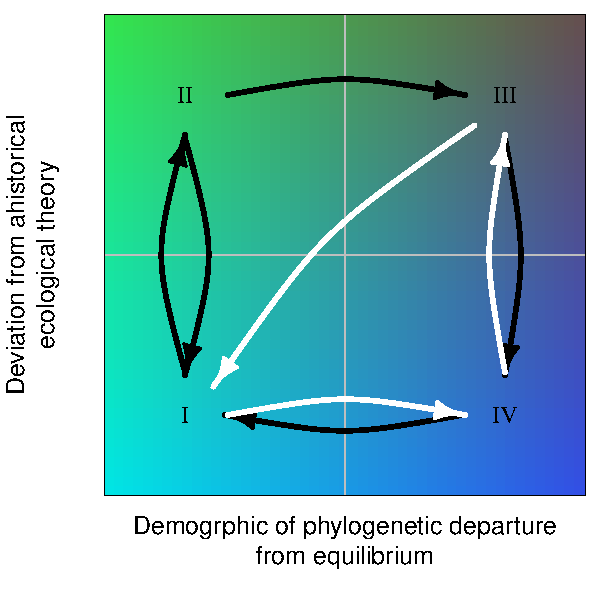
\includegraphics[scale=1]{fig_cycles.pdf}
  \caption{Hypothesized cycles between different states of equilibrium
    and non-equilibrium in ecological metrics (y-axis) and
    evolutionary metrics (x-axis). Panels I--IV are discussed in the
    next.  Colors correspond to deviation from ahistorical ecological
    theory and evolutionary equilibrium.  Black cycle corresponds to
    non-equilibrium initiated by ecological disturbance (with
    potential to continue to evolutionary non-equilibrium or
    relaxation to equilibrium). White cycle is initiated by
    evolutionary innovation.}
  \label{fig:cycles}
\end{figure}

\begin{figure}[!hbp]
  \centering
  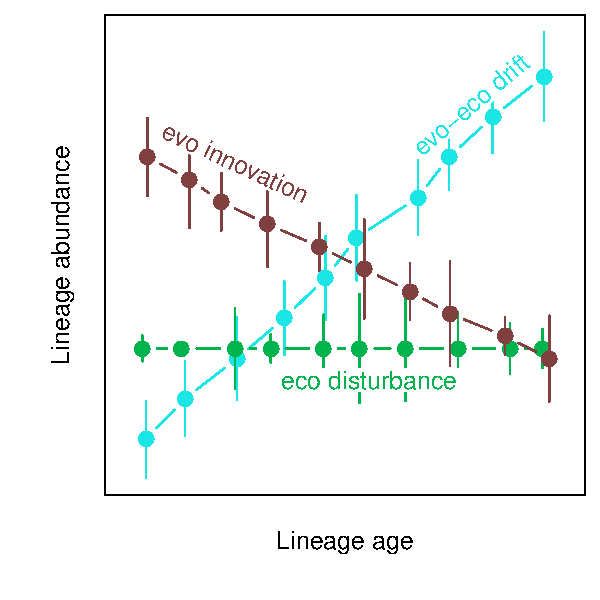
\includegraphics[scale=1]{fig_age-abund.pdf}
  \caption{Hypothesized relationships between lineage age and
    abundance under different evo-ecological scenarios. Colors
    correspond to panels in Figure \ref{fig:cycles}: teal is
    evo-ecological equilibrium; green is rapid transition to
    ecological non-equilibrium following short timescale distrubance;
    dark brown is non-equilibrium in both ecological and evolutionary
    metrics.}
  \label{fig:age-abund}
\end{figure}

\pagebreak

\section*{Box \ref{box:dry} figures}

\setcounter{figure}{0}
\renewcommand{\thefigure}{\Roman{figure}}

\begin{figure}[!hbp]
  \centering
  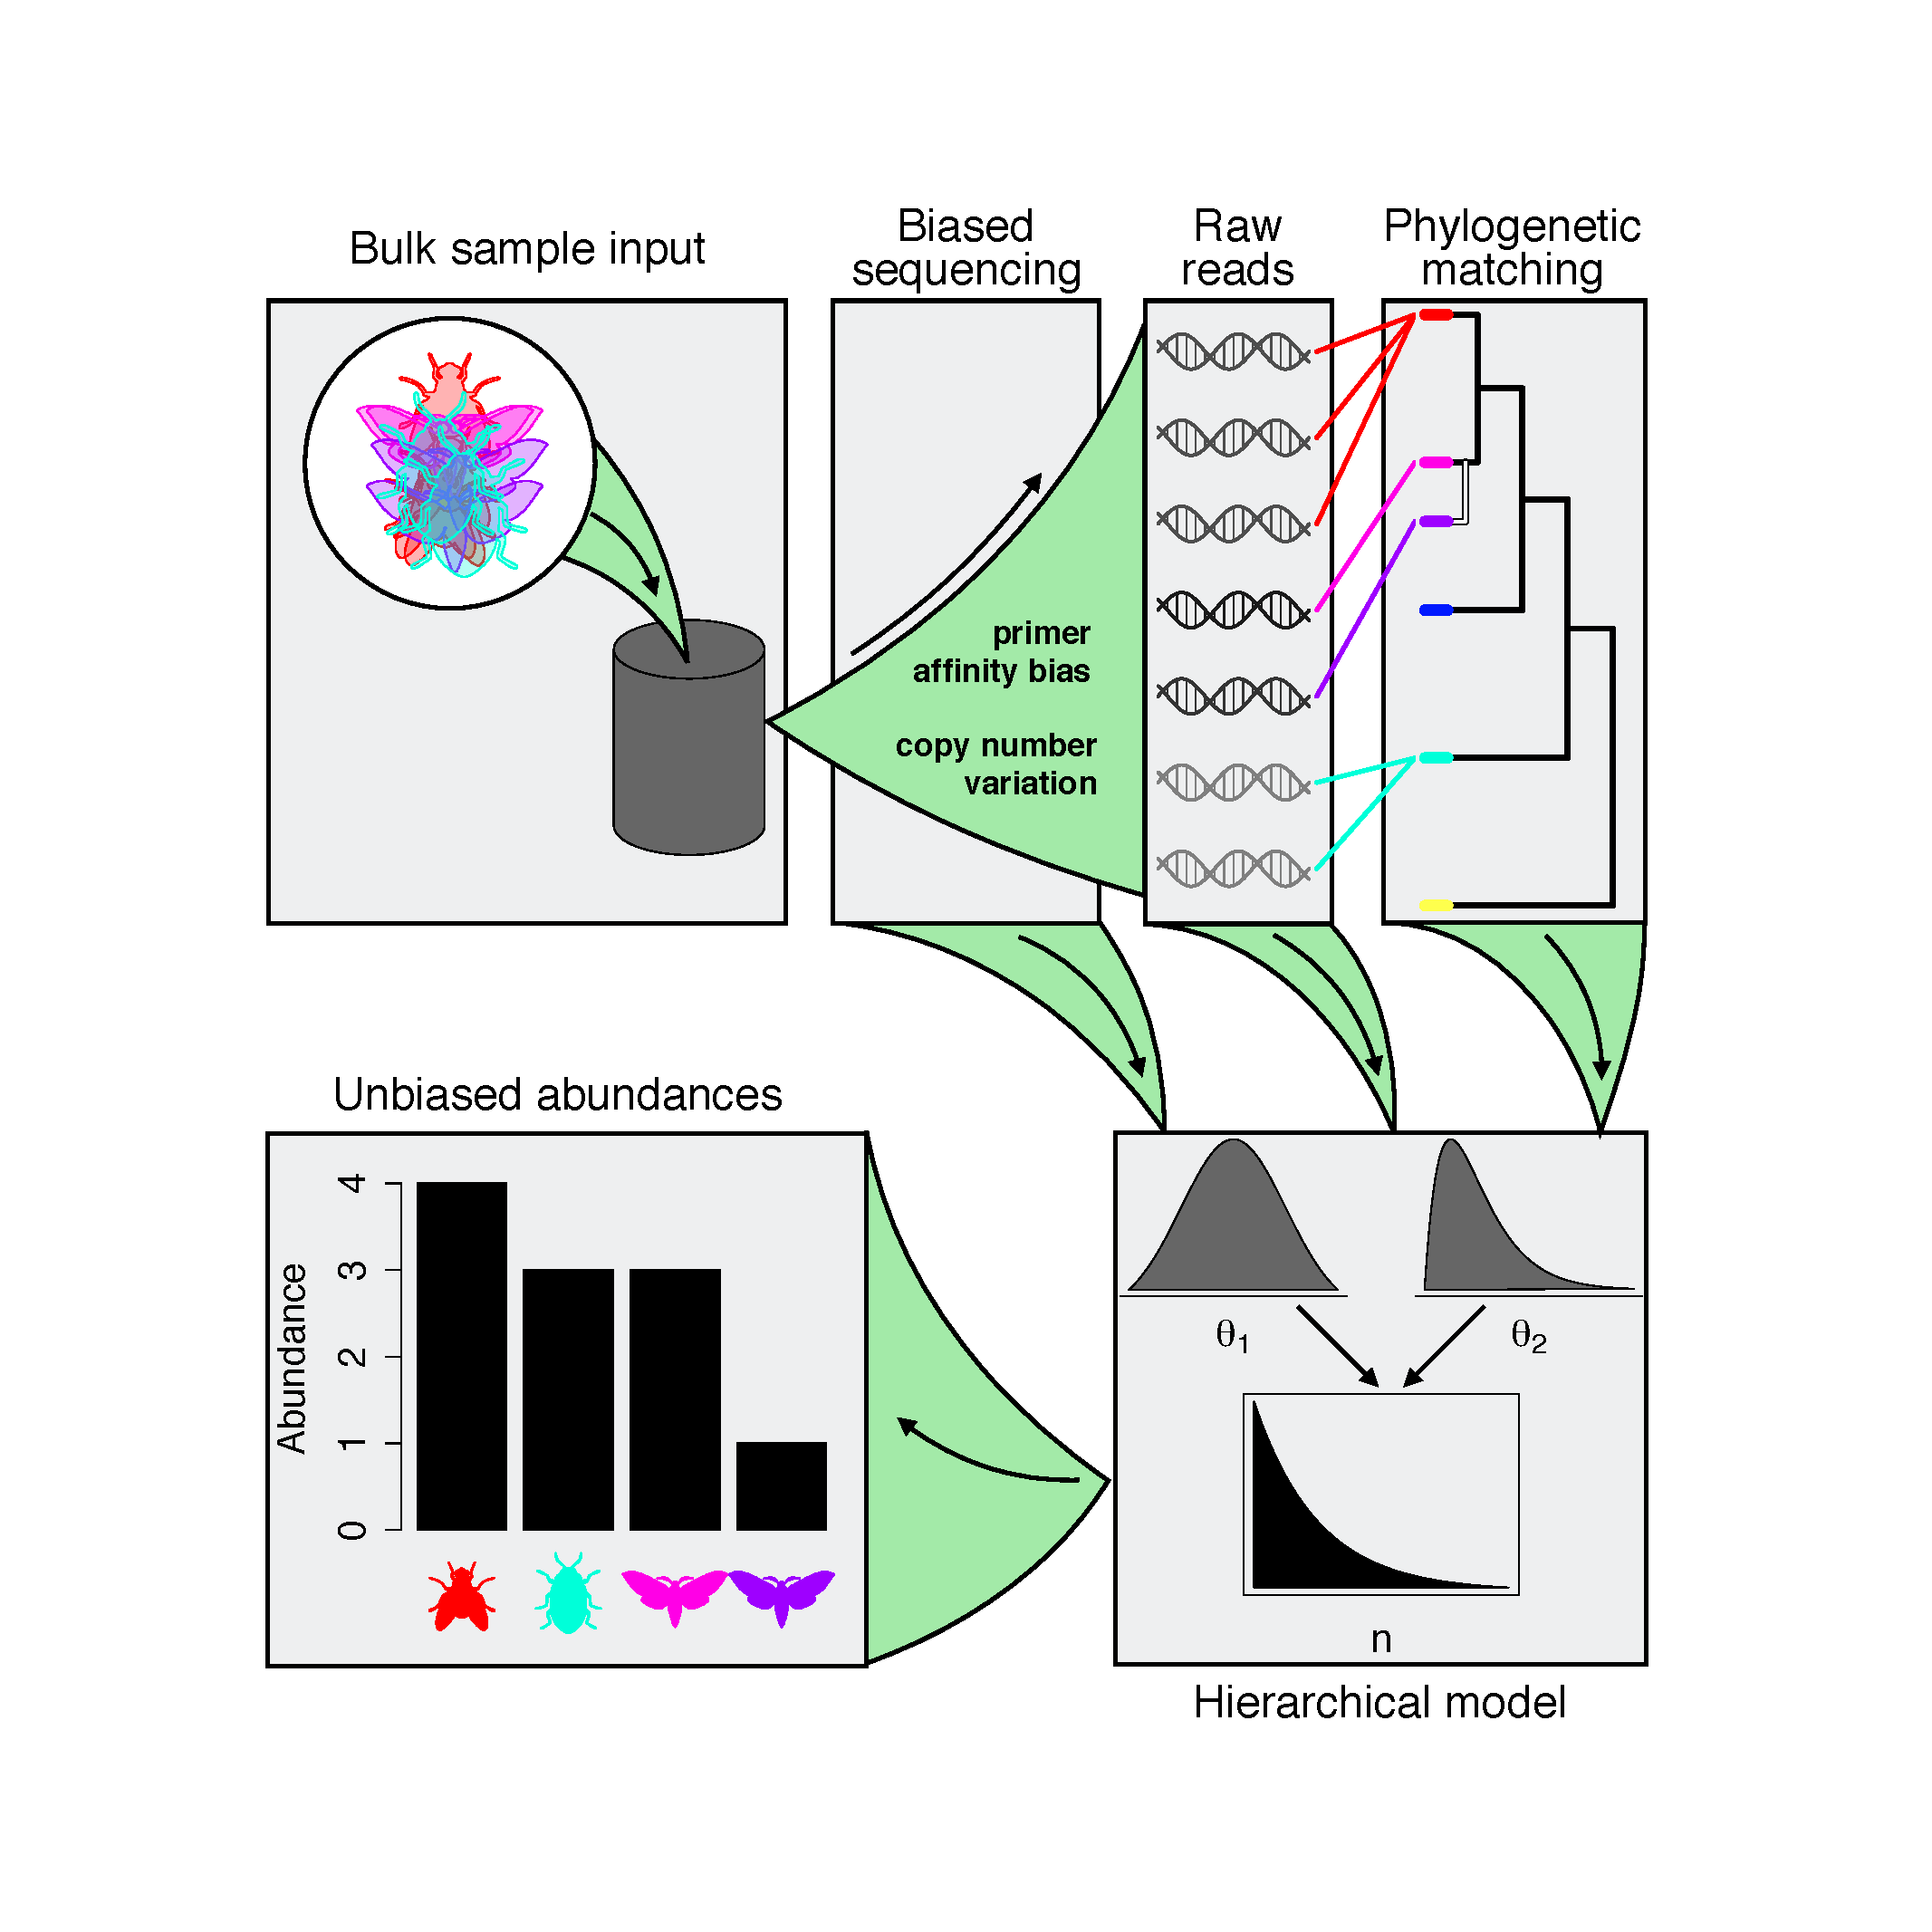
\includegraphics[scale=0.4]{fig_metab.pdf}
  \caption{Pipeline to estimate true abundances from metabarcoding
    data. The pipeline follows sequence generation, matching sequences
    to a phylogeny (generated from the sequences themselves, or better
    yet from highercoverage data) and finally Bayesian hierrarchical
    modeling leading to abundance estimates.}
  \label{fig:abundPipeline}
\end{figure}

\begin{figure}[!hbp]
  \centering
  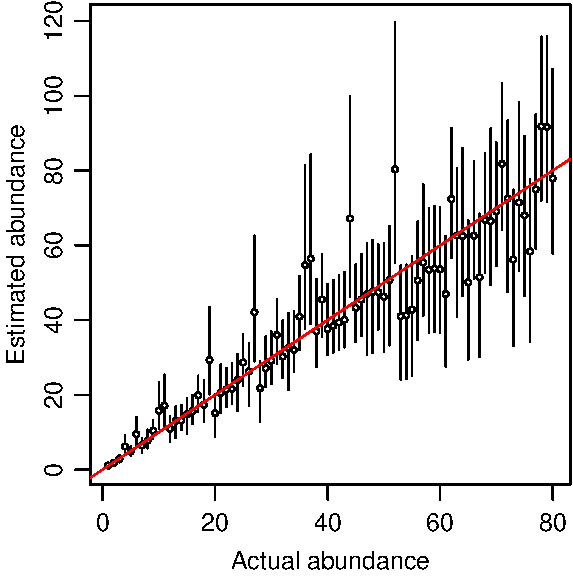
\includegraphics[scale=1]{fig_abundEst-1.pdf}
  \caption{Demonstration of agreement between actual and estimated
    abundances. Actual (simulated) abundances are on the x-axis, which
    the y-axis shows estimated abundances (error bars are 95\% maximum
    credible intervals). The simulation study is described in the
    supplement.}
  \label{fig:abundEst}
\end{figure}

\begin{figure}[!hbp]
  \centering
  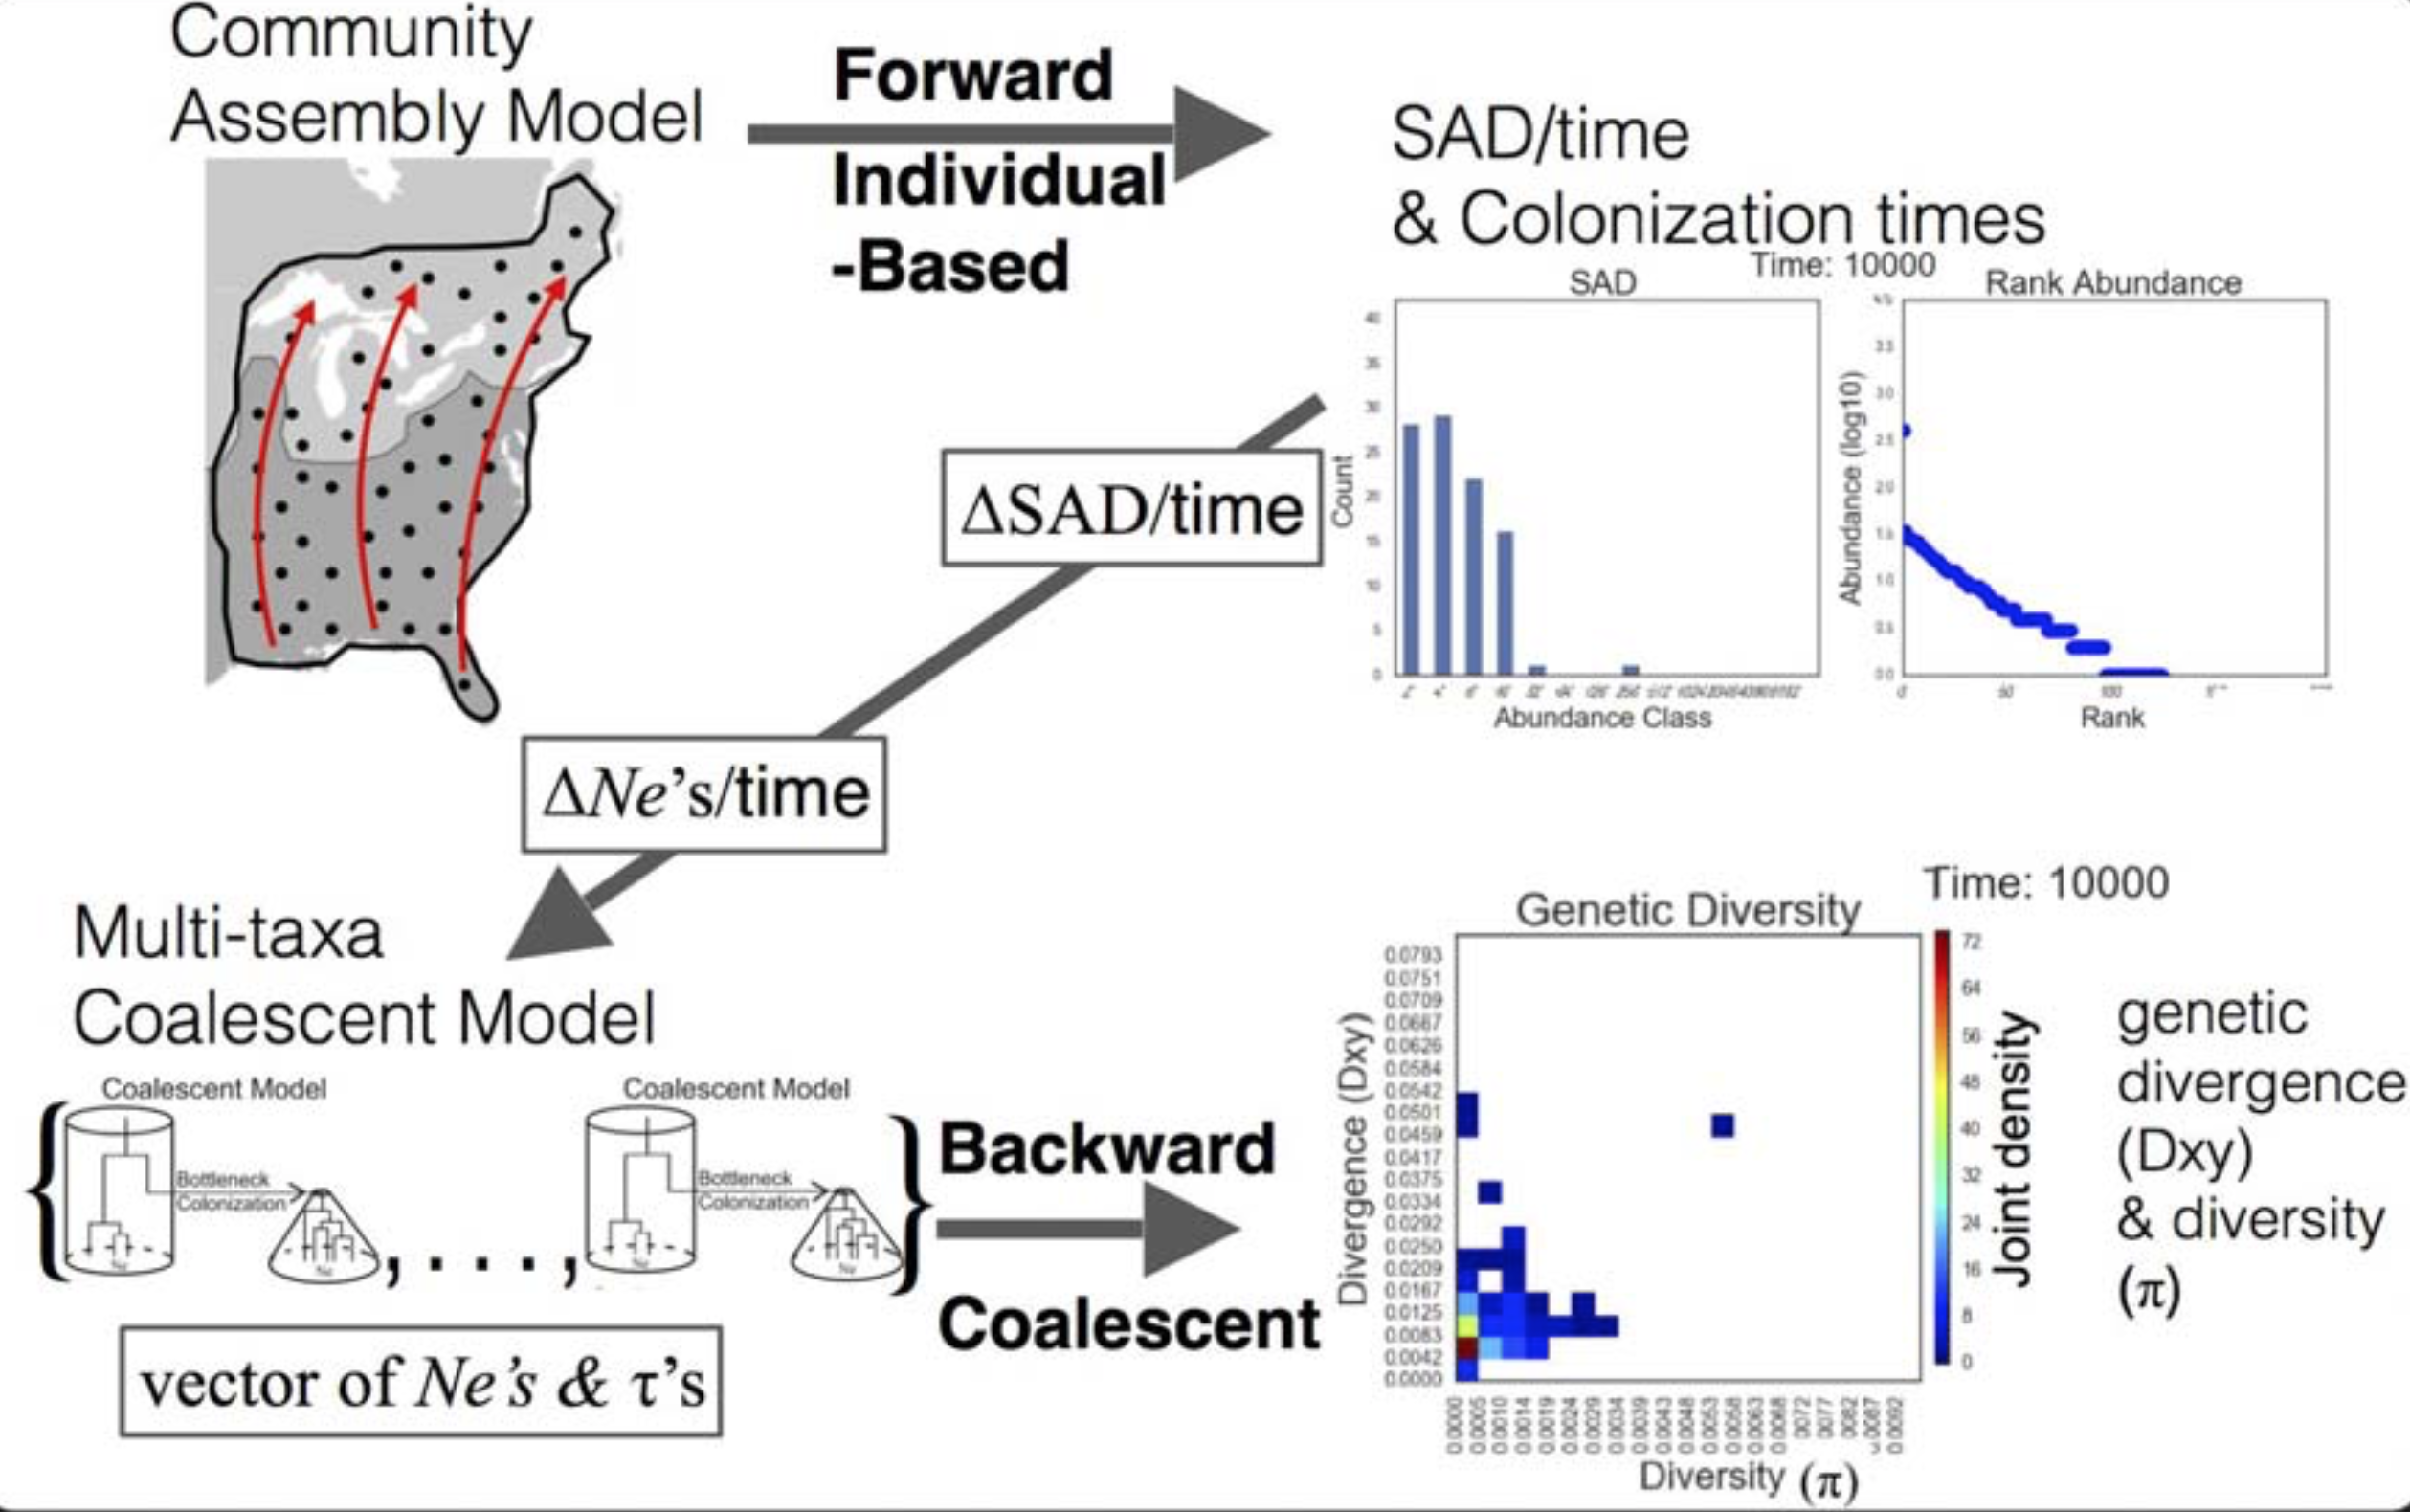
\includegraphics[scale=0.4]{fig_gimmeSAD.png}
  \caption{The gimmeSAD$\pi$ pipeline. The forward time models
    involves multi-regional expansion generating local abundance
    distributions over time with geterogeneity in
    colonizationtimes. These temporally dynamic local abundances are
    re-scaled into local $n_e$ distribuitons over time to generate
    multi-species genetic data the the coalescent, which is summarized
    here with a time-dependent joint spectrum of genetic diversity
    statistics.}
  \label{fig:gimmeSAD}
\end{figure}

\end{document}
